%
% Tutorial -- Active Filters Design with Qucs and Qucsactivefilter
%
% Copyright (C)  2014 Vadim Kuznetsov
%
% Permission is granted to copy, distribute and/or modify this document
% under the terms of the GNU Free Documentation License, Version 1.1
% or any later version published by the Free Software Foundation.
%

% redefine subfigure caption
\renewcommand{\thesubfigure}{\thefigure(\alph{subfigure})}
\makeatletter
  \renewcommand{\@thesubfigure}{\thesubfigure:\space}
  \renewcommand{\p@subfigure}{}
\makeatother

% redefine subtable caption
\renewcommand{\thesubtable}{\thetable(\alph{subtable})}
\makeatletter
  \renewcommand{\@thesubtable}{\thesubtable:\space}
  \renewcommand{\p@subtable}{}
\makeatother

\tutsection{Introduction}

The purpose of this manual is to explain bases of active filter design
methods using \verb|qucs-activefilter| tool. You can start
\verb|qucs-activefilter| by clicking in the Qucs main menu \emph{Tools->Active
Filters}. Qucsactivefilter provides easy and powerful tool for manipulations
with active filters. Qucsactivefilter can operate only active filters. For
passive filter use Qucsfilter instead. Basic explanations about active filters
could be found here: \url{https://en.wikipedia.org/wiki/Active_filter}

Qucsfilter builds active filters circuits based on RC-components and
operational amplifier (opamp). Qucsactivefilter uses ideal opamps.  It
uses 1-3 opamps per filter section. The number of opamps depends on selected
approximation type, filter type and topology.



\tutsection{Interface description}

The main window of this tool is shown in the Figure \ref{fig:mainwin}

\begin{figure}[ht]
  \centering
  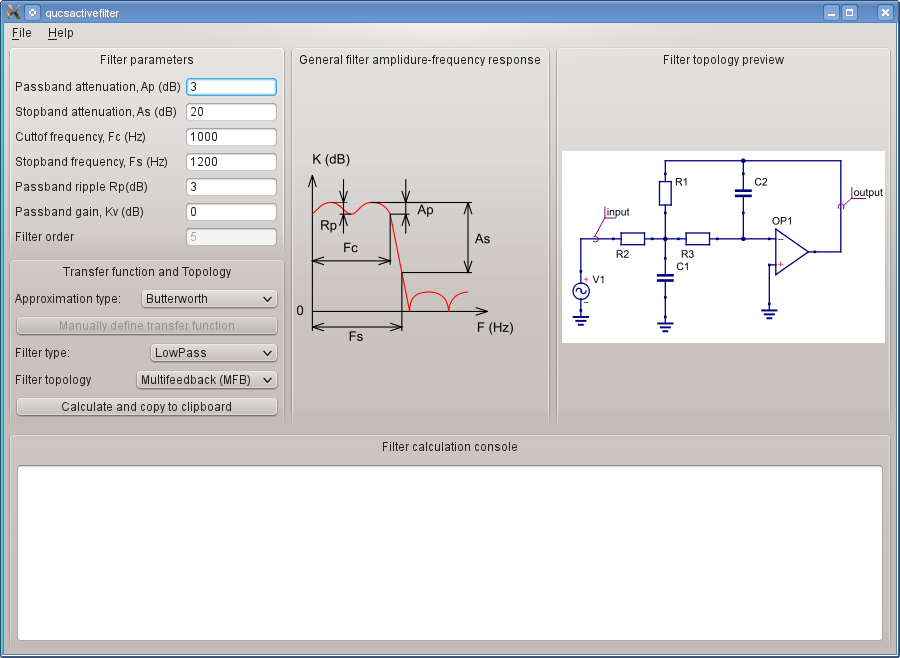
\includegraphics[width=\linewidth]{mainwindow}
  \caption{Qucs-Activefilter main window}
  \label{fig:mainwin}
\end{figure}
\FloatBarrier

Main windows contains five groups of controls: 

\begin{enumerate}
 \item Filter parameters input fields (left part of the window). You should
filter frequency response parameters here. These
parameters are shown on the frequency response preview. This part of the window
also contains \emph{Calculate and copy to clipboard} push button.
 \item Filter frequency response preview (middle part of the window). 
 \item Filter topology preview (right part of the window). You can see
common form of the filter section topology here.
 \item Calculation console. Filter order, poles/zeros list and part list are
printed here if filter calculation is successful. Part list contains
RC-elements values for each section of the filter.
 \item Menu bar. You can access \emph{File->Exit} and get short \emph{Help}
here.
\end{enumerate}

 

\tutsection{Filter transfer function}

Active filters are characterized by transfer function in frequency domain.
Common form of the filter transfer function is given here:

\begin{equation}
 H(s)=\frac{b_m s^m+b_{m-1}s^{m-1}+\ldots+b_2 s^2+b_1 s+b_0}
           {a_n s^n+a^{n-1}s^{n-1}+\ldots+a_2 s^2+a_1 s+a_0}
\end{equation}

Filter order $N$ is:

\begin{equation}
 N = \max(m,n)
\end{equation}

Filter order determines the number of filter sections and filter circuit
complexity. Active filter consists of $k=N/2$ 2-nd order section and $k=N\%2$
1-st order sections. 

Zeros of the transfer function are roots of numerator.  Poles are the roots of
denominator. We need to know filter transfer function to determine components
(resistors and capacitors --- RC) values of the active filter circuit.

Qucsactivefilter uses user-defined filter parameters in frequency domain to
determine filter order, transfer function and RC-elements value for each
section of the filter.

Qucsactivefilter uses filter design algorithms provided by [D. Johnson, J.
Johnson, H. Moore A handbook of active filters --- Prentice-Hall, Inc,
Engewood Cliffs., N.J.07632, USA, --- 1980].


\tutsection{Filters parameters explanation}

We need to define following four groups of parameters to calculate active
filter:

\begin{enumerate}
 \item Frequency response approximation type. Butterworth, Chebyshev,
Inverse Chebyshev,  Cauer (Elliptic), Legendre, and Bessel filters are 
available.
 \item Frequency response parameters: filter gain and bandwidth.
 \item Filter topology. Sallen-Key, Mutifeedback (MFB) and Cauer topologies are
available.
 \item Filter type. Low-pass, high-pass, band-pass and band-stop filters are
available.
\end{enumerate}

All of these parameters are presented in the left side of Qucsactivefilter main
window.

Different filter topologies have different number of opamps, resistors and
capacitors per section. Sallen-Key and MFB topologies are the most suitable for
Chebyshev and Butterworth filters.

Frequency response parameters differ for various filter types (low-pass,
high-pass, band-pass, band-stop) and approximations.


Frequency response of low-pass and high-pass filters has following
parameters:

\begin{enumerate}
 \item Cutoff frequency $F_c$
 \item Passband attenuation $A_p$
 \item Passband ripple $R_p$ (for Chebyshev and Cauer filters only)
 \item Stopband attenuation $A_s$
 \item Stopband frequency $F_s$
 \item Passband gain $K$
\end{enumerate}

Qucsactivefilter estimates filter order automatically for Chebyshev,
Butterworth and Cauer filter. Minimal order that provides required frequency
domain parameter is used. You don't need define filter order manually for these
approximations. filtersOrder could not be determined automatically for Bessel
filter. You should
define filer order for the Bessel and Legendre filters manually.

Frequencies should be defined in Hertz (Hz). Attenuation and ripple should
be defined in decibels (dB).

Frequency response of band-pass and band-stop filters has following
parameters:

\begin{enumerate}
 \item Upper cutoff frequency $F_u$
 \item Lower cutoff frequency $F_l$
 \item Transient bandwidth $TW$ is gap between pass band and stop band.
 \item Passband ripple $R_p$ (for Chebyshev and Cauer filters only)
 \item Stopband attenuation $A_s$
 \item Passband gain $K$
\end{enumerate}

Only Chebyshev, inverse Chebyshev and Cauer filters have ripple in pass band.
Butterworth and Bessel have no. Cauer filter has ripple in stop band too.
Qucsactivefilter suggests that stop band ripple less than stopband attenuation.

All of these parameters you can see in frequency response preview in the middle
part of the Qucsactivefilter main window.

\tutsection{Filter design example}

For example, consider Chebyshev low-pass filter with following parameters:

\begin{enumerate}
 \item Cutoff frequency: 2 kHz;
 \item Passband ripple: 2 dB;
 \item Stopband frequency: 2.2 kHz
 \item Stopband attenuation: 20 dB
 \item Passband gain: 0 dB
\end{enumerate}

At first step we need to put these parameters into corresponding input fields.
in the left part of the main window. Then we need to select Chebyshev
approximation in the \emph{Approximation type} combo box, select Sallen-Key
topology in \emph{Filter topology} combo box and select low-pass filter in
\emph{Filter type} combo box. The next figure presents main window with filled
input fields for our example.

\begin{figure}[ht]
  \centering
  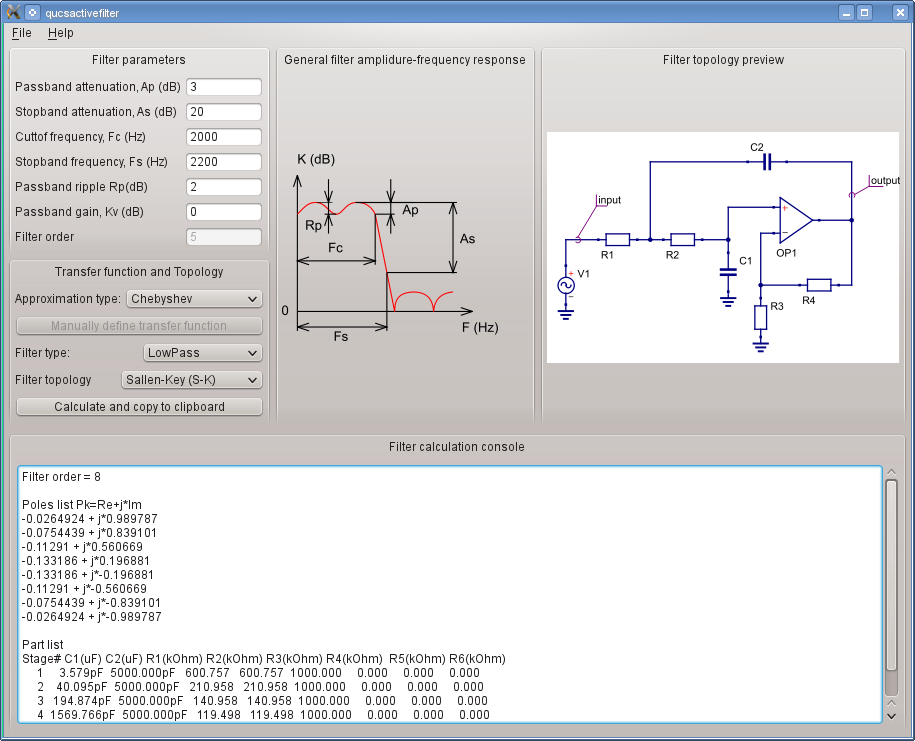
\includegraphics[width=\linewidth]{sk-2kHz}
  \caption{Sallen-Key low-pass filter design example with Qucsactivefilter}
  \label{fig:sk2kHz}
\end{figure}
\FloatBarrier

As all input fields are filled, we can press \emph{Calculate and copy to
clipboard} button. After this button is clicked, we can see calculation
results (transfer function poles and zeros list and part list) in the bottom
part of the main window. Filter is calculated successfully. If there was errors
during filter calculation, calculation process is aborted and warning message
box appears. You should change frequency response parameters and/or filter
topology in such case.

You can use components values from the part list for active filter simulation
with external circuit simulation program.


Now filter
schematic is in the system clipboard. We can switch back to the Qucs schematic
window and press Ctrl+V or \emph{Edit->Paste}. Filter schematic appears (Fig.
\ref{fig:sk2kHz-qucs})

\begin{figure}[!ht]
  \centering
  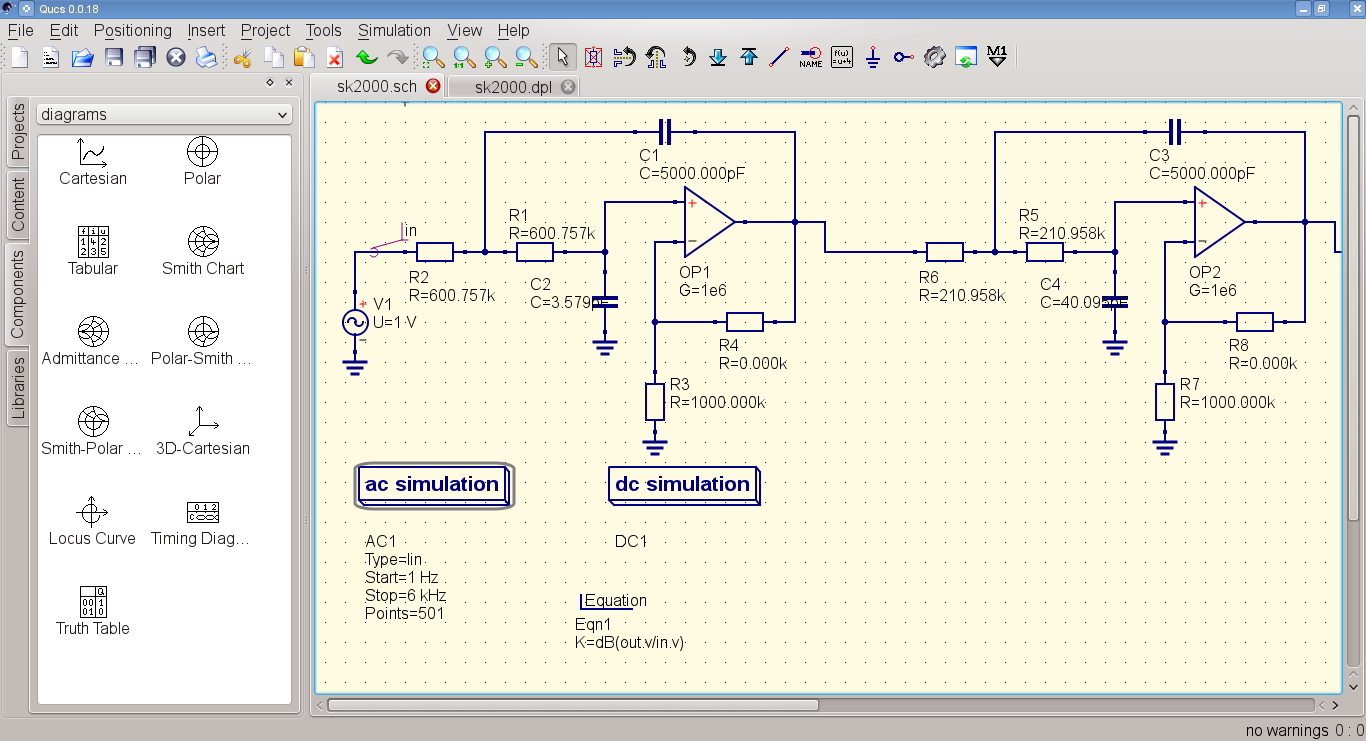
\includegraphics[width=\linewidth]{qucs-sk2kHz}
  \caption{Sallen-Key filter schematic in Qucs}
  \label{fig:sk2kHz-qucs}
\end{figure}
\FloatBarrier

This schematic already contains AC and DC simulations and equation for the
filter gain calculation ($K$ parameter). We can press F2 and simulate it.
Simulation completes and we can switch to the display page and place Cartesian
plot on it. If we place K graph on this plot, we can see frequency response of
the filter (Fig.\ref{fig:resp}). This frequency response meets all required
parameters.

\begin{figure}[!ht]
  \centering
  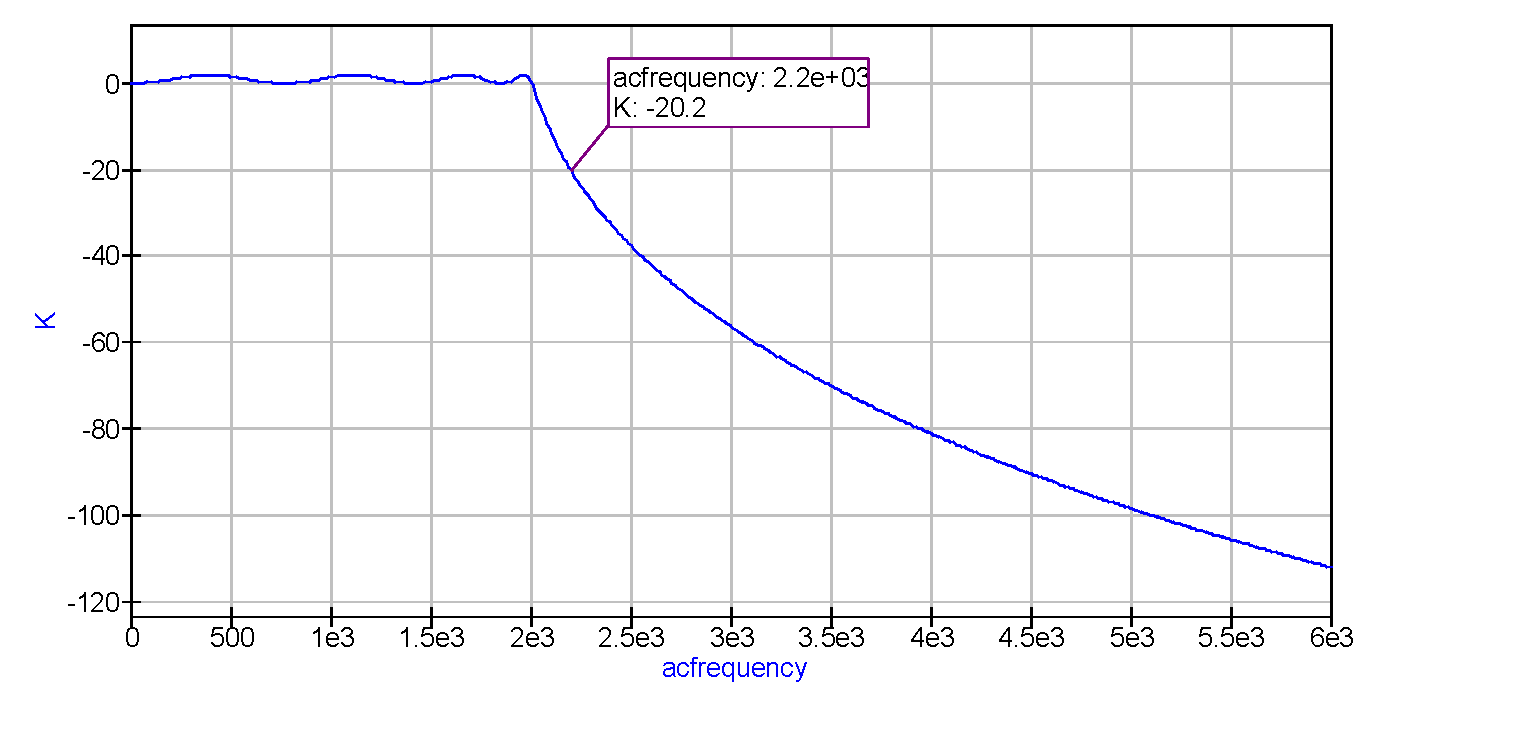
\includegraphics[width=0.9\linewidth]{response}
  \caption{Filter simulation results (frequency response)}
  \label{fig:resp}
\end{figure}
\FloatBarrier

\tutsection{Manual transfer function definition}

Using Qucsactivefilter you can define numerator and denominator coefficients
manually. It's need to select \emph{User defined} transfer function in
\emph{Approximation type} combo box. \emph{Manually define transfer function}
button becomes available. Transfer function setup dialog
(Fig.\ref{fig:mantrfunc})
appears after the click on this button.

\begin{figure}[ht]
  \centering
  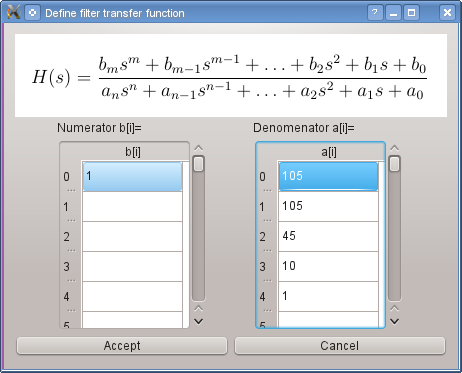
\includegraphics[width=0.6\linewidth]{manual-trfunc}
  \caption{Manual transfer function definition}
  \label{fig:mantrfunc}
\end{figure}
\FloatBarrier

You can fill two columns of the table and define numerator ($a_i$) and
denominator ($b_i$) transfer function coefficients. Then you can press
\emph{Accept} button and calculate active filter with given topology.

Presented example (Fig.\ref{fig:mantrfunc}) implements the following transfer
function:

\begin{equation}
 H(s)=\frac{1}{s^4+10s^3+45s^2+105s+105}
\end{equation}

This transfer function implements 4th-order Bessel filter.


\tutsection{Conclusion}

Qucsactivefilter tool was considered. You can easy design active filter with
this tool and Qucs. Report about any bugs  for Qucsactivefilter to Vadim
Kuznetsov (E-mail: \url{ra3xdh@gmail.com}).

